 
\documentclass[xcolor=pdftex,dvipsnames,table]{beamer}
\usepackage{etex}
% EEHPT: You can change the theme color from Green to other colors.
\usecolortheme[named=Blue]{structure}

\usetheme{CambridgeUS}
%\usefonttheme{serif}
\setbeamercovered{dynamic}
\usepackage{wrapfig}
\usepackage[absolute,overlay]{textpos}
\usepackage{verbatim}
%\usepackage{hyperref}
\usepackage{graphicx}
\usepackage{ifthen}

    \usepackage{tikz}
    \usetikzlibrary{arrows}
	\usetikzlibrary{decorations.pathreplacing}
	\usepackage{tikz-3dplot} %requires 3dplot.sty to be in same directory, or in your LaTeX installation
	
	
\usepackage{float}
\usepackage[export]{adjustbox}
\usepackage{bm}
\usepackage{amsmath}
\usepackage{hyperref}
\usepackage{booktabs}
\newtheorem{name}{Printed output}
\newtheorem{prop}{Proposition}
\newtheorem{assum}{Assumptions}
\newtheorem{defin}{Definitions}
\newtheorem{lemm}{Lemma}
\setbeamercovered{invisible}


\begin{document}

\title{Optimal Anti-Poverty Programs}
\subtitle{An Application to the Brazilian \textit{Bolsa Fam\'ilia}}
\author{Juan Rios}

\maketitle

\begin{frame}
 \frametitle{Motivation}
% EEHPT: Put content here (of course, you can make it more than one slide)
%\pause
\begin{itemize}
\item Cash transfer programs are common (Brazil, Chile, Mexico etc)
%\pause
\item \textit{Bolsa Fam\'ilia} is the largest Conditional Cash Transfer program in the world
\begin{itemize}
%\pause
\item 30 million beneficiaries as of March 2015
%\pause
\item Individuals below annual income of US\$ 528
\end{itemize}
\end{itemize}
\end{frame}

\begin{frame}[label=question]
 \frametitle{The Research Question}
% EEHPT: Put content here (of course, you can make it more than one slide)
\begin{itemize}
\item What is the benefit schedule that minimizes the cost of the program given a minimum consumption level?
%\pause
\begin{itemize}
\item Labor supply responses
\item Mis-reporting responses
\end{itemize}
%\pause
\item In this talk:
\begin{itemize}
\item What are the elasticities of reported and real income?
\end{itemize}
\end{itemize}
\hyperlink{literature}{\beamergotobutton{Link to Literature}}
\end{frame}

\begin{frame}
    \frametitle{Outline}
    \tableofcontents[pausesections]
\end{frame}

\section{Institutional Background}

\begin{frame}
	\frametitle{The \textit{Bolsa Fam\'ilia} Program}
	%\pause
\begin{itemize}
\item Benefits based on: 
\begin{itemize}
\item Household income per capita
\item Household Composition
\end{itemize}
%\pause
\item Information is collected in program's offices
\begin{itemize}
\item Assets, demographics and income are self-reported to interviewers
\item Interviewers may adjust the reported income
\item Computer calculates the per capita income
\end{itemize}
%\pause
\item Timing
\begin{itemize}
\item Interviews on any business day
\item Updates at least once every two years
\end{itemize}
%\pause
\item Audits
\begin{itemize}
\item Take away benefits
\item Vary with the gov. budget
\item Geographical variation
\end{itemize}
\end{itemize}	
\end{frame}

\begin{frame}
\frametitle{Households with 3 Members \only<-4>{and 1 Child} \only<5->{after Last Reform}}
\begin{center}
\scalebox{0.7}{
\begin{tikzpicture}[x=1.4,y=1.4]
\node[align=center, right] at (200,0) {$y$ (R\$)};
\draw[->, very thick] (0,0) -- (200,0) ; %edit here for the x axis
\node[align=center, above] at (0,200) {$y+B(y)$ (R\$)};
\draw[->, very thick] (0,0) -- (0,200) ; %edit here for the y axis

%\pause
\only<-4>{\draw[red!70!black, -, very thick] (0,30) -- (70,100) ; % 45 degree line
\draw[red!70!black, -, very thick] (70,100) -- (70,77.333) ; % notch
\draw[red!70!black, -, very thick] (70,77.333) -- (140,147.33) ; % 45 degree line
\draw[red!70!black, -, very thick] (140,147.33) -- (140,140) ; % notch
\draw[red!70!black, -, very thick] (140,140) -- (180, 180); % 45 degree line
\draw[red!70!black, -, very thick] (165,80) -- (180, 80);
\node[black, align=center, right] at (180,80) {07.30.2009};
\node[black, align=right, left] at (0,30) {\scriptsize{30}};
\draw[black, -, dashed, thick] (70,0) -- (70,77.333) ;
\node[black, align=center, below] at (70,0) {\scriptsize{70}};
\draw[black, -, dashed, thick] (140,0) -- (140,140) ;
\node[black, align=center, below] at (140,0) {\scriptsize{140}};}

\pause
\only<2-4>{\draw[green!70!black, -, very thick] (0,34) -- (70,104) ; % 45 degree line
\draw[green!70!black, -, very thick] (70,104) -- (70,80.666) ; % notch
\draw[green!70!black, -, very thick] (70,80.666) -- (140,150.666) ; % 45 degree line
\draw[green!70!black, -, very thick] (140,150.666) -- (140,140) ; % notch
\draw[green!70!black, -, very thick] (140,140) -- (180, 180); % 45 degree line
\draw[green!70!black, -, very thick] (165,90) -- (180, 90);
\node[black, align=center, right] at (180,90) {04.11.2011};
\node[black, align=right, left] at (0,34) {\scriptsize{34}};}

\pause
\only<3-4>{\draw[blue!70!black, -] (0,70) -- (36,70) ; % flat line
\draw[blue!70!black, -] (36,70) -- (70,104); % 45 degree line
\draw[blue!70!black, -] (70,104) -- (70,80.666) ; % notch
\draw[blue!70!black, -] (70,80.666) -- (140,150.666) ; % 45 degree line
\draw[blue!70!black, -] (140,150.666) -- (140,140) ; % notch
\draw[blue!70!black, -] (140,140) -- (180, 180); % 45 degree line

\draw[blue!70!black, -] (165,100) -- (180, 100);
\node[black, align=center, right] at (180,100) {06.18.2012};
%Note that this date should be adjusted to 11.18.2012 if child is older than 6 (but younger than 15)
\node[black, align=right, left] at (0,70) {\scriptsize{70}};}

\pause
\only<4->{\draw[black, -] (0,77) -- (39.666,77) ; % flat line
\draw[black, -] (39.666,77) -- (77,114.333); % 45 degree line
\draw[black, -] (77,114.333) -- (77,88.666) ; % notch
\draw[black, -] (77,88.666) -- (154,165.666) ; % 45 degree line
\draw[black, -] (154,165.666) -- (154,154) ; % notch
\draw[black, -] (154,154) -- (180, 180); % 45 degree line

\draw[black, -] (165,110) -- (180, 110);
\node[black, align=center, right] at (180,110) {\only<4>{06.01.2014}\only<5->{With Children}};
\node[black, align=right, left] at (0,77) {\scriptsize{77}};
\draw[black, -, dashed, thick] (77,0) -- (77,88.666) ;
\node[black, align=center, below] at (77,0) {\scriptsize{77}};
\draw[black, -, dashed, thick] (154,0) -- (154,154) ;
\node[black, align=center, below] at (154,0) {\scriptsize{154}};}
\pause
\pause
\only<5->{\draw[orange, -] (0,77) -- (51.333,77) ; % flat line
\draw[orange, -] (51.333,77) -- (77,102.666); % 45 degree line
\draw[orange, -] (77,102.666) -- (77,77) ; % notch
\draw[orange, -] (77,77) -- (180, 180); % 45 degree line

\draw[orange, -] (165,100) -- (180, 100);
\node[black, align=center, right] at (180,100) {Without Children};}
\end{tikzpicture}
}
\end{center}
\end{frame}

\section{Data}
\begin{frame}
	\frametitle{Data}
% EEHPT: Put content here (of course, you can make it more than one slide)
%\pause
\begin{itemize}
\item Bolsa Fam\'ilia Administrative Data for 2011-2015 (only 2015 today)
\begin{itemize}
\item Panel with the self-reported income 
\item Family Composition
\item Date of the Income Update
\end{itemize}
%\pause
\item RAIS
\begin{itemize}
\item Universe of all formal employees in Brazil from 2002-2014
\item Monthly income 
\item Individual level identifier
\end{itemize}
\end{itemize}
\end{frame}

\begin{frame}
\begin{table}[htbp]
  \centering
  \caption{Selection}
    \begin{tabular}{crr|r}
\toprule
 & Only BF & Formal Empl. & Total \\
\midrule
Individuals & 2560438 & 455495 & 3015933 \\
 & (     84.9\%) & (     15.1\%) & (100\%) \\
Hhs (1 formal empl) & 634088 & 359267 & 993355 \\
 & (     63.8\%) & (     36.2\%) & (100\%) \\
Hhs (All formal empl) & 746007 & 247348 & 993355 \\
 & (     75.1\%) & (     24.9\%) & (100\%) \\
\bottomrule
\end{tabular}

  \label{tab_selection}%
\end{table}%
\end{frame}

\begin{frame}[label=ybar0]
\frametitle{Reported Income Distribution (0 children)}
\begin{figure}[H]
\begin{center}
\includegraphics[height=2.7in]{Dom_060114_non_0_bin3p5.pdf}
\end{center}
\end{figure}
\hyperlink{ybar0_sel}{\beamergotobutton{Link Selected Sample}}
\end{frame}

\begin{frame}[label=ybar2]
\frametitle{Reported Income Distribution (2 children)}
\begin{figure}[H]
\begin{center}
\includegraphics[height=2.7in]{Dom_060114_non_2_bin3p5.pdf}
\end{center}
\end{figure}
\hyperlink{ybar2_sel}{\beamergotobutton{Link to Selected Sample}}
\end{frame}

\begin{frame}
\frametitle{3rd Party Reported Income Distribution (0 children)}
\begin{figure}[H]
\begin{center}
\includegraphics[height=2.7in]{Rais_060114_non_0_bin3p5.pdf}
\end{center}
\end{figure}
\end{frame}

\begin{frame}
\frametitle{3rd Party Reported Income Distribution (2 children)}
\begin{figure}[H]
\begin{center}
\includegraphics[height=2.7in]{Rais_060114_non_2_bin3p5.pdf}
\end{center}
\end{figure}
\end{frame}

\section{Elasticities Estimation}

\begin{frame}[label=schedule]
\frametitle{Program Schedule}
\begin{center}
\begin{tikzpicture}[x=.9,y=.9]
\node[align=center, right] at (200,0) {$\bar{y}$};
\draw[->, very thick] (0,0) -- (200,0) ; %edit here for the x axis
\node[align=center, above] at (0,200) {$\bar{y}+B(\bar{y})$};
\draw[->, very thick] (0,0) -- (0,200) ; %edit here for the y axis

\draw[black, -, thick] (0,37.333) -- (77,114.333); % 45 degree line
\draw[black, -, thick] (77,114.333) -- (77,88.666) ; % notch
\draw[black, -, thick] (77,88.666) -- (154,165.666) ; % 45 degree line
\draw[black, -, thick] (154,165.666) -- (154,154) ; % notch
\draw[black, -, thick] (154,154) -- (180, 180); % 45 degree line

\draw[black, -, dashed, thick] (77,0) -- (77,88.666) ;
\node[black, align=center, below] at (77,0) {\scriptsize{77}};
\draw[black, -, dashed, thick] (154,0) -- (154,154) ;
\node[black, align=center, below] at (154,0) {\scriptsize{154}};
%\pause
\draw[-, thick] (0,37.333) -- (10,37.333) ;
\draw (10,37.333) arc (0:45:10);
\node[black, align=center, right] at (10,42.333) {\scriptsize{$1+B'(\bar{y})=1$}};
%\pause
\node[black, align=center, right] at (170,100) {\scriptsize{$\bar{e}=\frac{\partial \bar{y}}{\partial B'}\frac{1+B'}{\bar{y}}$ is not recoverable}};
\end{tikzpicture}
\end{center}
\end{frame}

\begin{frame}
\frametitle{Adjusted Bunching Method}
%\pause
\begin{align*}
U(\bar{y},\tilde{y};e,\tilde{e},n)=\bar{y}+\tilde{y}+B(\bar{y})-\frac{n}{1+1/e}\left(\frac{\bar{y}+\tilde{y}}{n}\right)^{1+1/e}-\frac{\tilde{y}^{1+1/\tilde{e}}}{1+1/\tilde{e}}
\end{align*}
pause
\begin{itemize}
\item $\bar{y}$: Reported Income
\item $\tilde{y}$: Hidden Income
\item $y=\bar{y}+\tilde{y}$: Real Income
\item $n$: Ability 
%\pause
\item $e=\frac{1+B'}{y}\frac{\partial y}{\partial B'}$: Elasticity of Real Income
\item $\tilde{e}=\frac{1}{\tilde{y}}\frac{\partial \tilde{y}}{\partial B'}$: Hidden Income Response
%\pause
\item $\bar{e}=\frac{1+B'}{\bar{y}}\frac{\partial \bar{y}}{\partial B'}=\frac{1+B'}{\bar{y}}\left(	\frac{y}{1+B'}e-\tilde{y}\tilde{e}\right)$: Elasticity of Reported Income
\end{itemize}
\end{frame}

\begin{frame}
\frametitle{Usual Bunching}
\begin{center}
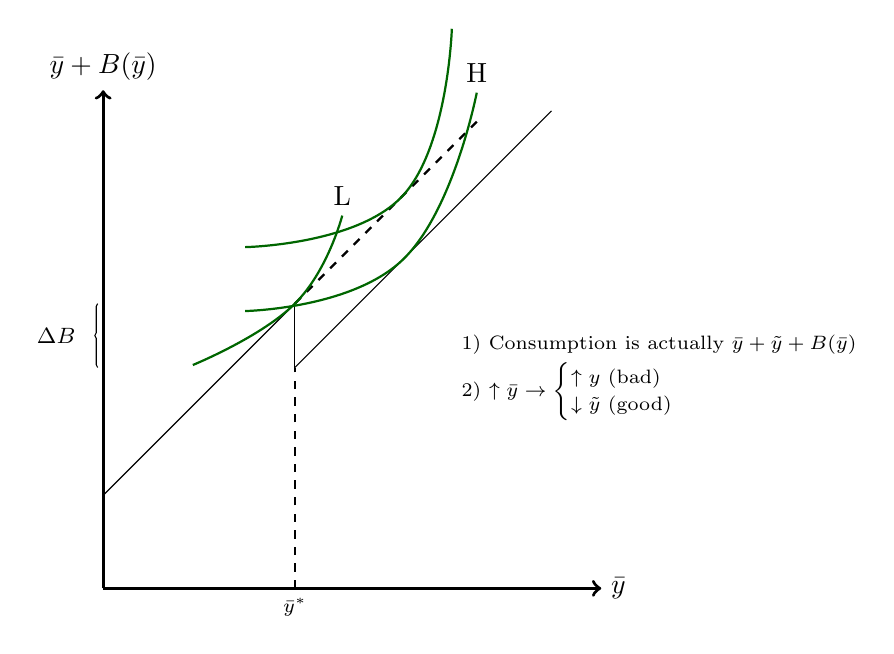
\begin{tikzpicture}[x=.9,y=.9]
\node[align=center, right] at (200,0) {$\bar{y}$};
\draw[->, very thick] (0,0) -- (200,0) ; %edit here for the x axis
\node[align=center, above] at (0,200) {$\bar{y}+B(\bar{y})$};
\draw[->, very thick] (0,0) -- (0,200) ; %edit here for the y axis

\draw[black, -] (0,37.333) -- (77,114.333); % 45 degree line
\draw[black, -] (77,114.333) -- (77,88.666) ; % notch
\draw[black, -] (77,88.666) -- (180,191.666) ; % 45 degree line
\draw [decorate,decoration={brace,amplitude=1pt},xshift=-2pt,yshift=0pt]
(0,88.666) -- (0,114.333)node [black,midway,xshift=-15pt] {\footnotesize $\Delta B$};


\draw[black, -, dashed, thick] (77,114.333) -- (150,187.333) ;

\draw[black, -, dashed, thick] (77,0) -- (77,88.666) ;
\node[black, align=center, below] at (77,0) {\scriptsize{$\bar{y}^*$}};

\draw [green!40!black, thick] plot [smooth, tension=.8] coordinates { (36,89.666) (77,114.333) (96,149.666)};
\node[align=center, above] at (96,149.666) {L};
\draw [green!40!black, thick] plot [smooth, tension=.8] coordinates {(57,111.333)  (120,131.666) (150,199)};
\draw [green!40!black, thick] plot [smooth, tension=.8] coordinates {(57,137)  (120,157.333) (140,224.666)};
\node[align=center, above] at (150,199) {H};


%\pause
\node[black, align=center, right] at (140,98){\scriptsize{1) Consumption is actually $\bar{y}+\tilde{y}+B(\bar{y})$}};
%\pause
\node[black, align=center, right] at (140,79){\scriptsize{2) $ \uparrow \bar{y} \rightarrow \begin{cases}\uparrow y \text{ (bad)}\\ \downarrow \tilde{y} \text{ (good)}\end{cases}$}};

\end{tikzpicture}
\end{center}
\end{frame}

\begin{frame}
\frametitle{Adjusted Bunching Method (Reported Income)}
\begin{center}
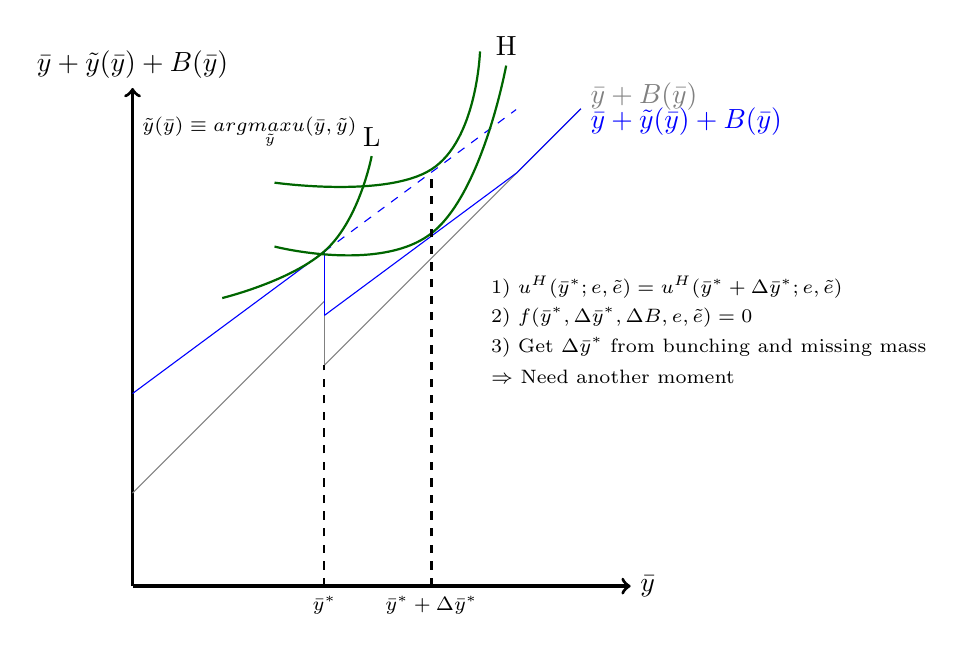
\begin{tikzpicture}[x=.9,y=.9]
\node[align=center, right] at (200,0) {$\bar{y}$};
\draw[->, very thick] (0,0) -- (200,0) ; %edit here for the x axis
\node[align=center, above] at (0,200) {$\bar{y}+\tilde{y}(\bar{y})+B(\bar{y})$};
\draw[->, very thick] (0,0) -- (0,200) ; %edit here for the y axis

\draw[gray, -] (0,37.333) -- (77,114.333); % 45 degree line
\draw[gray, -] (77,114.333) -- (77,88.666) ; % notch
\draw[gray, -] (77,88.666) -- (180,191.666) ; % 45 degree line
\node[gray, align=center, right] at (180,196.666) {$\bar{y}+B(\bar{y})$};

\draw[black, -, dashed, thick] (77,0) -- (77,88.666) ;
\node[black, align=center, below] at (77,0) {\scriptsize{$\bar{y}^*$}};

\node[black, align=center, right] at (0,182){\scriptsize{$\tilde{y}(\bar{y})\equiv arg\underset{\tilde{y}}{max}u(\bar{y},\tilde{y})$}};
%\pause

\draw[blue, -] (0,77.333) -- (77,134.333); 
\draw[blue, -, dashed] (77,134.333) -- (154,191.333) ; 
\draw[blue, -] (77,134.333) -- (77,108.666) ; % notch
\draw[blue, -] (77,108.666) -- (154.333,166) ; 
\draw[blue, -] (154.333,166) -- (180,191.666);
\node[blue, align=center, right] at (180,186.666) {$\bar{y}+\tilde{y}(\bar{y})+B(\bar{y})$};

%\pause

\draw [green!40!black, thick] plot [smooth, tension=.8] coordinates { (36,115.666) (78,135.333) (96,172.666)};
\node[align=center, above] at (96,172.666) {L};
%\pause
\draw [green!40!black, thick] plot [smooth, tension=.8] coordinates {(57,136.333)  (120,141.666) (150,209)};
\draw [green!40!black, thick] plot [smooth, tension=.8] coordinates {(57,162)  (120,167.333) (139.5,214.666)};
\node[align=center, above] at (150,209) {H};

\draw[black, -, dashed, thick] (120,0) -- (120,166.333) ;
\node[black, align=center, below] at (120,0) {\scriptsize{$\bar{y}^*+\Delta \bar{y}^*$}};

%\pause
\node[black, align=center, right] at (140,120){\scriptsize{1) $u^H(\bar{y}^*;e,\tilde{e})=u^H(\bar{y}^*+\Delta \bar{y}^*;e,\tilde{e})$}};
%\pause
\node[black, align=center, right] at (140,108){\scriptsize{2) $f(\bar{y}^*, \Delta \bar{y}^*, \Delta B, e, \tilde{e})=0$}};
%\pause
\node[black, align=center, right] at (140,96){\scriptsize{3) Get $\Delta \bar{y}^*$ from bunching and missing mass}};
\node[black, align=center, right] at (140,84){\scriptsize{$\Rightarrow$ Need another moment}};

\end{tikzpicture}
\end{center}
\end{frame}

\begin{frame}
\frametitle{Adjusted Bunching Method (Real Income)}
\begin{center}
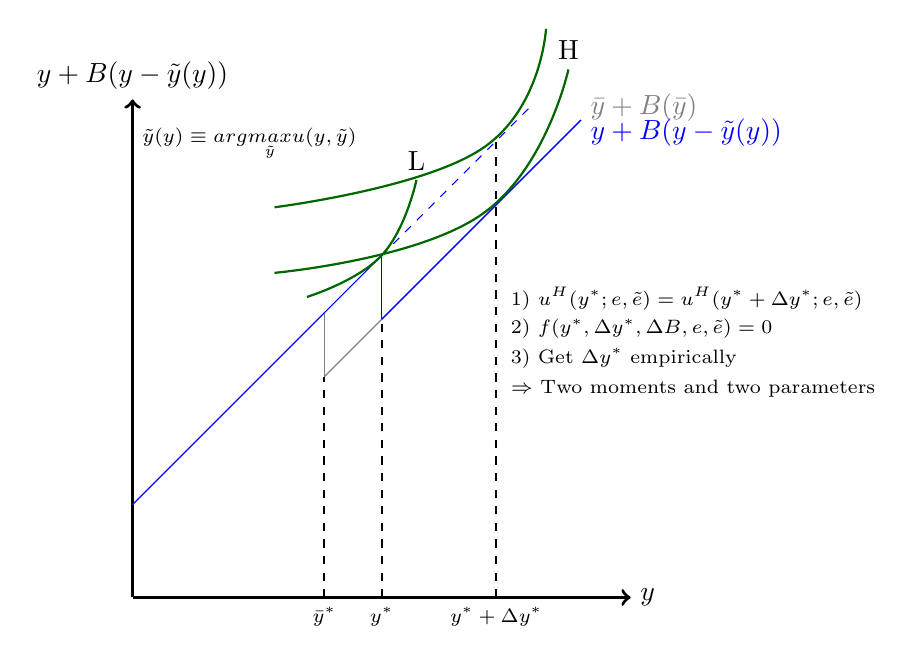
\begin{tikzpicture}[x=.9,y=.9]
\node[align=center, right] at (200,0) {$y$};
\draw[->, very thick] (0,0) -- (200,0) ; %edit here for the x axis
\node[align=center, above] at (0,200) {$y+B(y-\tilde{y}(y))$};
\draw[->, very thick] (0,0) -- (0,200) ; %edit here for the y axis

\node[black, align=center, right] at (0,182){\scriptsize{$\tilde{y}(y)\equiv arg\underset{\tilde{y}}{max}u(y,\tilde{y})$}};

\draw[gray, -] (0,37.333) -- (77,114.333); % 45 degree line
\draw[gray, -] (77,114.333) -- (77,88.666) ; % notch
\draw[gray, -] (77,88.666) -- (180,191.666) ; % 45 degree line
\node[gray, align=center, right] at (180,196.666) {$\bar{y}+B(\bar{y})$};

\draw[black, -, dashed, thick] (77,0) -- (77,88.666) ;
\node[black, align=center, below] at (77,0) {\scriptsize{$\bar{y}^*$}};

%\pause

\draw[blue, -] (0,37.333) -- (100,137.333); 
\draw[blue, -, dashed] (100,137.333) -- (160,197.333) ; 
\draw[blue, -] (100,137.333) -- (100,111.666) ; % notch
\draw[blue, -] (100,111.666) -- (180,191.666);
\node[blue, align=center, right] at (180,186.666) {$y+B(y-\tilde{y} (y))$};
\draw[black, -, dashed, thick] (100,0) -- (100,111.666) ;
\node[black, align=center, below] at (100,0) {\scriptsize{$y^*$}};
%\pause

\draw [green!40!black, thick] plot [smooth, tension=.8] coordinates { (70,120.666) (100,137.333) (114,167.666)};
\node[align=center, above] at (114,167.666) {L};
%\pause
\draw [green!40!black, thick] plot [smooth, tension=.8] coordinates {(57,130.333)  (140,153.666) (175,212)};
\draw [green!40!black, thick] plot [smooth, tension=.8] coordinates {(57,156.666)  (140,180) (166,228.333)};
\node[align=center, above] at (175,212) {H};

\draw[black, -, dashed, thick] (146,0) -- (146,183) ;
\node[black, align=center, below] at (146,0) {\scriptsize{$y^*+\Delta y^*$}};
%\pause
\node[black, align=center, right] at (148,120){\scriptsize{1) $u^H(y^*;e,\tilde{e})=u^H(y^*+\Delta y^*;e,\tilde{e})$}};
%\pause
\node[black, align=center, right] at (148,108){\scriptsize{2) $f(y^*, \Delta y^*, \Delta B, e, \tilde{e})=0$}};
%\pause
\node[black, align=center, right] at (148,96){\scriptsize{3) Get $\Delta y^*$ empirically}};
\node[black, align=center, right] at (148,84){\scriptsize{$\Rightarrow$ Two moments and two parameters}};
\end{tikzpicture}
\end{center}
\end{frame}

\begin{frame}[label=discretized]
\frametitle{Discretized Program Schedule}
\begin{center}
\begin{tikzpicture}[x=.9,y=.9]
\node[align=center, right] at (200,0) {$w_i$};
\draw[->, very thick] (0,0) -- (200,0) ; %edit here for the x axis
\node[align=center, above] at (0,200) {$c_i=w_i+B_i$};
\draw[->, very thick] (0,0) -- (0,200) ; %edit here for the y axis

\fill (0,37.333) circle (1.5);
\fill (7,44.333) circle (1.5);
\fill (14,51.333) circle (1.5);
\fill (21,58.333) circle (1.5);
\fill (28,65.333) circle (1.5);
\fill (35,72.333) circle (1.5);
\fill (42,79.333) circle (1.5);
\fill (49,86.333) circle (1.5);
\fill (56,93.333) circle (1.5);
\fill (63,100.333) circle (1.5);
\fill (70,107.333) circle (1.5);
\fill (77,114.333) circle (1.5);

\fill (84,95.666) circle (1.5);
\fill (91,102.666) circle (1.5);
\fill (98,109.666) circle (1.5);
\fill (105,116.666) circle (1.5);
\fill (112,123.666) circle (1.5);
\fill (119,130.666) circle (1.5);
\fill (126,137.666) circle (1.5);
\fill (133,144.666) circle (1.5);
\fill (140,151.666) circle (1.5);
\fill (147,158.666) circle (1.5);
\fill (154,165.666) circle (1.5);

\fill (161,161) circle (1.5);
\fill (168,168) circle (1.5);
\fill (175,175) circle (1.5);
\fill (182,182) circle (1.5);
\fill (189,189) circle (1.5);
\fill (196,196) circle (1.5);
\fill (203,203) circle (1.5);

%\pause

\draw [decorate,decoration={brace,amplitude=1pt},xshift=-2pt,yshift=0pt]
(0,37.333) -- (0,44.333)node [black,midway,xshift=-15pt] {\footnotesize $c_1-c_0$};
\draw[black, -, dashed] (0,44.333) -- (7,44.333) ;

%\pause
\draw [decorate,decoration={brace,amplitude=1pt},xshift=-2pt,yshift=0pt]
(0,95.666) -- (0,114.333)node [black,midway,xshift=-25pt] {\footnotesize $-(c_{12}-c_{11})$};
\draw[black, -, dashed] (0,114.333) -- (77,114.333) ;
\draw[black, -, dashed] (0,95.666) -- (84,95.666) ;

%\pause
\draw [decorate,decoration={brace,amplitude=1pt},xshift=-2pt,yshift=0pt](0,161) -- (0,165.666)node [black,midway,xshift=-25pt] {\footnotesize $-(c_{23}-c_{22})$};
\draw[black, -, dashed] (0,165.666) -- (154,165.666) ;
\draw[black, -, dashed] (0,161) -- (161,161) ;

%\pause

\node[black, align=center, right] at (150,100) {\scriptsize{$\bar{\mathcal{E}}_i=\frac{\partial \bar{h}_i}{\partial (c_i-c_{i-1})}\frac{(c_i-c_{i-1})}{\bar{h}_i}$ is recoverable}};
\node[black, align=center, right] at (150,80) {\scriptsize{$\mathcal{\bar{E}}_i(w_i-w_{i-1})=\bar{e}_iw_i$}};
\end{tikzpicture}
\end{center}
\hyperlink{proof_relation}{\beamergotobutton{Link to Proof}}
\end{frame}

\begin{frame}[label=empirical]
\frametitle{Empirical Strategy}
\begin{itemize}
\item $y_{jt}$: Income reported by household $j$ in period $t$.
\pause
\item $y^*_{jt}$: Latent income, so that $y_{jt}=\begin{cases}y^*_{jt}\ if\ y^*_{jt}>0\\
0\ if\ y^*_{jt}\leq 0 \end{cases}$
\pause
\item $\Delta y_j = y_{jt_1}-y_{jt_0}$
\pause
\item $\delta \equiv med(\Delta y_j)$: Income bracket width
\pause
\begin{center}
\scalebox{0.65}{
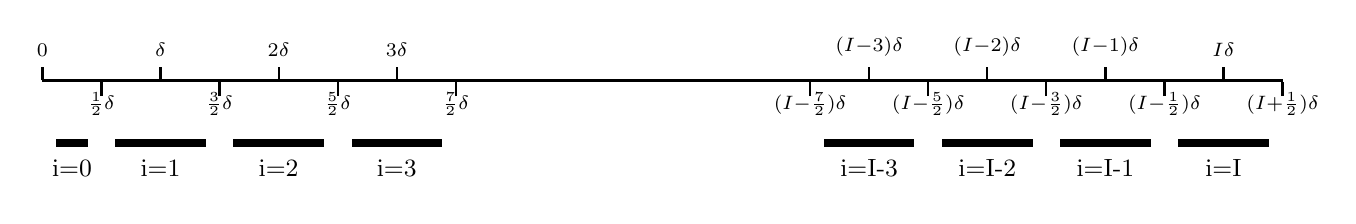
\begin{tikzpicture}[x=1.5cm]
\draw[black,-,thick,>=latex]
(0,0) -- (10.5,0) node[below right] {$\scriptstyle$};

\draw[black,thick] 
( 0,0) -- ++(0,5pt) node[above] {$\scriptstyle 0$};
\draw[black,thick] 
( 1,0) -- ++(0,5pt) node[above] {$\scriptstyle \delta$};

\foreach \Xc in {2,3}
{
  \draw[black,thick] 
    ( \Xc,0) -- ++(0,5pt) node[above] {$\scriptstyle \Xc \delta$};
}

\foreach \Xc/\texto in {7/(I-3)\delta,8/(I-2)\delta,9/(I-1)\delta,10/I\delta}
{
  \draw[black,thick] 
    ( \Xc,0) -- ++(0,5pt) node[above] {$\scriptstyle \texto$};
}

\foreach \Xc/\texto in {0.5/\frac{1}{2},1.5/\frac{3}{2},2.5/\frac{5}{2},3.5/\frac{7}{2}}
{
  \draw[black,thick] 
    ( \Xc,-.2) -- ++(0,5pt) node[below] {$\scriptstyle \texto \delta$};
}
\foreach \Xc/\texto in {6.5/(I-\frac{7}{2}),7.5/(I-\frac{5}{2}),8.5/(I-\frac{3}{2}),9.5/(I-\frac{1}{2}),10.5/(I+\frac{1}{2})}
{
  \draw[black,thick] 
    ( \Xc,-.2) -- ++(0,5pt) node[below] {$\scriptstyle \texto \delta$};
}
  \fill[black] 
    ([xshift=5pt]0,-0.75)  
      rectangle node[below] {\strut\small i=0} 
    ([xshift=-5pt]0.5,-0.85);  
\foreach \Xc/\Texto in {0.5/i=1,1.5/i=2,2.5/i=3}
{
  \fill[black] 
    ([xshift=5pt]\Xc,-0.75)  
      rectangle node[below] {\strut\small\Texto} 
    ([xshift=-5pt]\Xc+1,-0.85);  
}
\foreach \Xc/\Texto in {6.5/i=I-3,7.5/i=I-2,8.5/i=I-1,9.5/i=I}
{
  \fill[black] 
    ([xshift=5pt]\Xc,-0.75)  
      rectangle node[below] {\strut\small\Texto} 
    ([xshift=-5pt]\Xc+1,-0.85);  
}
\end{tikzpicture} 
}
\end{center}
\item $d_{ij}=\begin{cases}1 & \text{if hh $j$ can report $0$, $i-1$ or $i$},\\
0 & \text{otherwise.} \end{cases}$  ``intrinsic" occupation
\pause
\item $h_{ijt}=\begin{cases}1\ & \text{hh $j$ reports $i$ in $t$},\\
0 & \text{otherwise.} \end{cases}$ ``equilibrium" occupation
\end{itemize}
\end{frame}

\begin{frame}[label = identification1]
\frametitle{Identifying $\eta_i=\frac{\partial h_i}{\partial(c_i-c_0)}\frac{c_i-c_0}{h_i}$ and $\mathcal{E}_i=\frac{\partial h_i}{\partial(c_i-c_{i-1})}\frac{c_i-c_{i-1}}{h_i}$}
\begin{itemize}
\item $y^*_{jt}=\sum_{i=1}^I d_{ij}(w_i*h_{i,j,t}+ w_{i-1}* h_{i-1,j,t})+u_{jt},$
\pause
\item $h_{ijt}=\begin{cases}1$ if $h_{ijt}^*>0\\
0$ otherwise,$\end{cases}\ where\ h^*_{ijt}=f(\underbrace{(c_i-c_0),(c_i-c_{i-1})}_{X_{jt}})+\epsilon_{ijt},$
\pause
\item $E(h_{ijt}|X_{jt})=Prob(h_{ijt}^*=1|X_{jt})=Prob\Big(\epsilon_{ijt}>-f(X_{ijt})\Big)=1-G\Big(f(X_{ijt})\Big)$
\pause
\item $\Rightarrow h_{ijt}=1-G(f(X_{ijt}))+\nu_{ijt}$
\pause
\item $y^*_{jt}=\sum_{i=1}^I \beta_i d_{ij}ln(c_i-c_{i-1})_{jt}+\sum_{i=1}^I \gamma_i d_{ij}ln(c_i-c_{0})_{jt}+v_{jt}$\\
\pause
\item $d_{ij}$ defined empirically as a function of hh's composition, education, location and housing infrastructure.\hyperlink{intrinsic}{\beamergotobutton{Link to Intrinsic}}
\pause
\item $\frac{\beta_i}{w_i}=\eta_i\text{ and }\frac{\gamma_i}{\delta}=\eta_i$
\end{itemize}
\end{frame}

\begin{frame}[label=identification2]
\begin{block}

\textbf{Identification Assumption:} Labor supply and Mis-reporting decisions are not correlated with unobservables that changed with the program schedule.
\end{block}
\pause
\frametitle{Identifying $\eta_i=\frac{\partial h_i}{\partial(c_i-c_0)}\frac{c_i-c_0}{h_i}$ and $\mathcal{E}_i=\frac{\partial h_i}{\partial(c_i-c_{i-1})}\frac{c_i-c_{i-1}}{h_i}$}
\begin{itemize}
\item $v_{jt}=u_{jt}+\sum_{i=1}^I(\beta_i+\gamma_i)\nu_{ijt}*d_{ij}$
\begin{block}

\textbf{Tobit Assumption:} $u_{jt}\sim N(0,1)$
\end{block}
\item $L(B)=\prod_{j=1}^N\prod_{t=1}^T\Big\{\phi\left(y_{jt}-X_{jt}B+(\beta_i+\gamma_i)G(X_{jt})\right)[1-G(X_{jt})]$
$\phi\left(y_{jt}-X_{jt}B-(\beta_i+\gamma_i)[1-G(X_{jt})]\right)G(X_{jt})\Big\}$
\end{itemize} 
\hyperlink{timing}{\beamergotobutton{Link to Timing}}
\end{frame}

\section{Implications for the Optimal Program}

\begin{frame}[label=implications]
\frametitle{Optimality of the Anti-Poverty Program}
\begin{itemize}
%\pause
\item If there are no fines $\Rightarrow$ elasticities of reported income are sufficient statistics
%\pause
\item If there are fines $\Rightarrow$ elasticities of reported \underline{and real} income are sufficient statistics
%\pause
\item These are elasticities \underline{under the optimal schedule}
%\pause
\item The elasticities \underline{under the observed schedule} are sufficient statistics for the \underline{optimal reform}
\end{itemize}
\hyperlink{theory}{\beamergotobutton{Link to Discrete Model}}
\hyperlink{imp}{\beamergotobutton{Link to the Government's Problem}}
\hyperlink{prop_imp}{\beamergotobutton{Link to the Optimal Program}}
\hyperlink{reform}{\beamergotobutton{Link to the Optimal Reform}}
\end{frame}

\begin{frame}
\begin{figure}[H]
\begin{center}
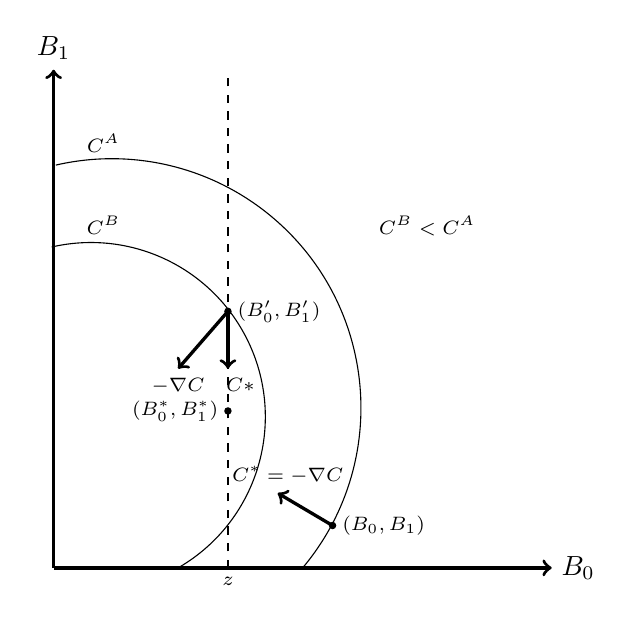
\begin{tikzpicture}[x=.9,y=.9]
\node[align=center, right] at (200,0) {$B_0$};
\draw[->, very thick] (0,0) -- (200,0) ; %edit here for the x axis
\node[align=center,  above] at (0,200) {$B_1$};
\draw[->, very thick] (0,0) -- (0,200) ; %edit here for the y axis
\draw (100,0) arc (-40:103:100);
\node[black, align=center, below] at (20,178) {\scriptsize{$C^A$}};
\draw (50,0) arc (-60:103:70);
\node[black, align=center, below] at (20,145) {\scriptsize{$C^B$}};
\node[black, align=center, below] at (150,145) {\scriptsize{$C^B<C^A$}};
%\pause
\draw[black, -, dashed, thick] (70,0) -- (70,200) ;
\node[black, align=center, below] at (70,0) {\scriptsize{$z$}};
%\pause
\fill (70,63) circle (1.5);
\node[black, align=center, left] at (70,63) {\scriptsize{$(B_0^*,B_1^*)$}};
%\pause
\fill (112,17) circle (1.5);
\node[black, align=center, right] at (112,17) {\scriptsize{$(B_0,B_1)$}};
%\pause
\draw[->, very thick] (112,17) -- (90,30) ; %edit here for the x axis
\node[black, align=center, above] at (94,30) {\scriptsize{$C^*=-\nabla C$}};
%\pause
\fill (70,103) circle (1.5);
\node[black, align=center, right] at (70,103) {\scriptsize{$(B'_0,B'_1)$}};
%\pause
\draw[->, very thick] (70,103) -- (50,80) ; %edit here for the x axis
\node[black, align=center, below] at (50,80) {\scriptsize{$-\nabla C$}};
%\pause
\draw[->, very thick] (70,103) -- (70,80) ; %edit here for the x axis
\node[black, align=center, below] at (75,80) {\scriptsize{$C*$}};

\end{tikzpicture}
\label{opt_reform}
\end{center}
\end{figure}
\end{frame}

\begin{frame}
\frametitle{Recap}
\begin{itemize}
%\pause
\item Recover elasticities of reported and real income from bunching in both distributions
%\pause
\item Those elasticities are the sufficient statistics for the Optimal Anti-Poverty program
%\pause
\item The optimal reform can be written as a function of elasticities under the observed schedule
\end{itemize}
\end{frame}

\appendix
\newcounter{finalframe}
\setcounter{finalframe}{\value{framenumber}}

\begin{frame}[label=literature]
 \frametitle{Related Literature}
% EEHPT: Put content here (of course, you can make it more than one slide) 
\begin{enumerate}
\item Taxable Income Elasticity Estimation
\begin{itemize}
\item Disentangle real responses from mis-reporting responses
\item Correction for the bunching estimation
\end{itemize}
%\pause
\item Optimal Income Maintenance Programs (Kanbur and Stern 1987, Kanbur et al 1994, Besley and Coate 1992 and 1995, Kleven and Kopczuk 2011)
\begin{itemize}
\item Bring this discussion to the data 
\item Incorporate extensive margin responses
\end{itemize}
%\pause
\item Modern Optimal Tax (Saez 2001 and 2002, Rotschild and Scheuer 2013 and 2015,  and Lockwood 2015, Huang and Rios 2015)
\begin{itemize}
\item Framework more relevant for developing countries 
\item Optimal reform as a function of elasticities under the observed schedule.
\end{itemize}
%\pause
\item Taxation in Developing Countries (Gordon and Li 2009, Best et al 2014, Pomeranz 2013, Naritomi 2015, Bachas and Soto 2015, )
\begin{itemize}
\item Focus here on cash-transfer programs (negative taxes).
\end{itemize}
\end{enumerate}
\hyperlink{question}{\beamergotobutton{Back to Research Question}}
\end{frame}

\begin{frame}[label=ybar0_sel]
\frametitle{Reported Income  (0 children) - Selected Sample}
\begin{figure}[H]
\begin{center}
\includegraphics[height=2.7in]{Dom1_060114_non_0_bin3p5.pdf}
\end{center}
\end{figure}
\hyperlink{ybar0}{\beamergotobutton{Back to Households with 0 Children}}
\end{frame}

\begin{frame}[label=ybar2_sel]
\frametitle{Reported Income (2 children) - Selected Sample}
\begin{figure}[H]
\begin{center}
\includegraphics[height=2.7in]{Dom1_060114_non_2_bin3p5.pdf}
\end{center}
\end{figure}
\hyperlink{ybar2_sel}{\beamergotobutton{Back to Complete Sample}}
\end{frame}

\begin{frame}[label=theory]
 \frametitle{Theoretical Framework}
 \begin{center}
$U^E=w_{\bar{i}+\tilde{i}}+B_{\bar{i}}-p_{\bar{i}}f_{\tilde{i}}-\psi(\bar{i}+\tilde{i},\tilde{i},m)$ 
 \end{center}
%\pause
\begin{itemize}
\item $\bar{i}$: reported income level 
\item $\tilde{i}$: hidden income level $\Rightarrow \bar{i}+\tilde{i}$ real income level
\item $w_0=0<w_1<...<w_I$: wages in each income level 
%\pause
\item $B_0,B_1,...,B_I$: Benefits for each reported level
%\pause
\item $p_{\bar{i}}$: probability of being audited if reports $\bar{i}$
\item $f_{\tilde{i}}$: fine of hiding $\tilde{i}$
%\pause
\item $\psi(\cdot,\cdot,m)$: Labor supply and misreporting costs of types $m$.
\end{itemize}
%\pause
 \begin{assum}
\begin{enumerate}
\item No income effect. 
\item Expected utility 
\item Some types cannot work
%\pause
\item Type $m$ reports either level $0$, $i(m)-1$ or $i(m)$:
\end{enumerate}
\end{assum}
\hyperlink{implications}{\beamergotobutton{Back to Implications}}
\end{frame}

\begin{frame}[label=imp]
 \frametitle{Cost Minimizing Objective}
\begin{itemize}
\item $\bar{h}_i$: Proportion of households reporting level $i$ in equilibrium
\item $\tilde{h}_i$: Proportion of households producing $i$ but reporting $i-1$.
\item $\tilde{H}_i$: Proportion of households producing $i$ but reporting $0$.
%\pause
\item $c_i=w_i+B_i$: Consumption observed by the government
%\pause
\item $z$: Minimum Consumption Level.
%\pause
\begin{align*}
	\underset{\{B_i\}_{i=0}^I}{min} \sum_{i=0}^I \{\bar{h}_iB_i-p_{i-1}f_1\tilde{h}_i-p_0f_i\tilde{H}_i\} \nonumber\\
	st\ c_0 \geq z\ and\ B_i\geq0\ \forall i. \nonumber
\end{align*}
\end{itemize}
\end{frame}

\begin{frame}[label=elasticities]
\begin{defin}
	Reported income elasticity in the extensive margin:
	\begin{align*}
	\bar{\eta}_i \equiv \frac{c_i-c_0}{\bar{h}_i}\frac{\partial \bar{h}_i}{\partial (c_i-c_0)},
\end{align*}
Reported income elasticity in the intensive margin:
\begin{align*}
	\bar{\mathcal{E}}_i \equiv \frac{c_i-c_{i-1}}{\bar{h}_i}\frac{\partial \bar{h}_i}{\partial (c_i-c_{i-1})}.
\end{align*}
\end{defin}
\end{frame}

\begin{frame}
$h_i$: Proportion of households producing $i$.
%\pause
\begin{defin}
	Real income elasticity in the extensive margin:
	\begin{align*}
	\eta_i \equiv \frac{c_i-c_0}{h_i}\frac{\partial h_i}{\partial (c_i-c_0)},
\end{align*}
Real income elasticity in the intensive margin:
\begin{align*}
	\mathcal{E}_i \equiv \frac{c_i-c_{i-1}}{h_i}\frac{\partial h_i}{\partial (c_i-c_{i-1})}.
\end{align*}
\end{defin}
\hyperlink{implications}{\beamergotobutton{Back to Implications}}
\end{frame}

\begin{frame}[label=prop_imp]
\begin{prop}
	\label{prop_imp_tra}
	Assuming that $\hat{\eta}^{*}_i\leq \frac{c^*_i-z}{z}$ for $i\geq v$, the cost minimizing schedule $\{B^*_i\}_{i=0}^I$ is: 
	\begin{align*}
	B_0^* = z \nonumber\\		
	\frac{B_i^*-B_{i-1}^*}{c^*_i-c^*_{i-1}}=-\frac{1}{\hat{\mathcal{E}}^*_i}\sum_{j=i}^{I}\left(\bar{h}^*_j+\hat{\eta}^*_i\frac{B_j^*-z}{c^*_j-z}\right)\	 for\ i =1,...,v-1  \nonumber\\
	B^*_i = 0\ for\ i = v, v+1, ...,I. \nonumber
	\end{align*}
	Where $\hat{\eta}^*_i\equiv(1-M_{\bar{n}(i)})h^*_i\eta^{*}_i+M_{\bar{n}(i)}\bar{h}^*_i\bar{\eta}^*_i$, 
	$\hat{\mathcal{E}}^*_i\equiv(1-\mu_{\bar{m}(i)})h^*_i\mathcal{E}^{*}_i+\mu_{\bar{m}(i)}\bar{h}^*_i\bar{\mathcal{E}}^*_i$ and $v$ is the smallest $i$ such that the $B^*_i$ implied by the second bracket is less or equal to zero. 
\end{prop}
\hyperlink{implications}{\beamergotobutton{Back to Implications}}
\hyperlink{proof_main}{\beamergotobutton{Link to Proof}}
\hyperlink{lemma}{\beamergotobutton{Link to Lemma}}
\hyperlink{welfare}{\beamergotobutton{Link to Welf Prob}}
\hyperlink{efficiency}{\beamergotobutton{Link to Efficiency}}
\begin{block}

\textbf{Problem:} Elasticities under the optimal schedule $\Rightarrow$ Non-recoverable.
\end{block}
\end{frame}

\begin{frame}[label=reform]
\begin{prop}
The cost minimizing local reform is a vector of perturbation in the benefit schedule $\Delta B = -(C_0,..,C_I)$ where:
	\begin{align*}				
	 C_0 =\begin{cases}\bar{h}_0-\sum_{i=1}^{v-1}\frac{B_i-B_0}{c_i-c_0}\hat{\eta}_i\ & if\ B_0>z\\
	 0\ & if\ B_0=z \end{cases}\\
	 C_i =\bar{h}_i+\frac{B_i-B_0}{c_i-c_0}\hat{\eta}_i+\frac{B_i-B_{i-1}}{c_i-c_{i-1}}\hat{\mathcal{E}}_i-\frac{B_{i+1}-B_{i}}{c_{i+1}-c_{i}}\hat{\mathcal{E}}_{i+1}\ 1\leq i\leq v\\ for\ \ i =1,...,v-1\\
	 C_{i} =min\left\{\bar{h}_{i}-\frac{B_0}{c_{i}-c_0}\hat{\eta}_{i}-\frac{B_{i-1}}{c_{i}-c_{i-1}}\hat{\mathcal{E}}_{i},0\right\}\ for\ i=v,...,I
	\end{align*}
	 $v$: lowest level with zero benefits
\end{prop}	
%\pause
\begin{block}

\textbf{Here all the parameters are recoverable from the data.}
\end{block}
\hyperlink{implications}{\beamerbutton{Back to Implications}}
\end{frame}

\begin{frame}[label=proof_main]
\begin{proof}
Since there are households that cannot work $\Rightarrow B_0^*=z$ \\
%\pause
Consider the perturbation at the optimum $dB_i=dB_{i+1}=...=dB_I=dB$. \\
\begin{enumerate}
%\pause
\item $ME =  dB\sum_{j=i}^Ih_j$.\\
%\pause
\item $BEIM = dh^{int}_i(B_i-B_{i-1})= (dk^{int}_i-de_i)(B_i-B_{i-1})$\\
%\pause
\item $BEEM = \sum_{j=i}^Idh^{ext}_j(B_j-B_0) =\sum_{j=i}^I(dk^{ext}_j-dE_j)(B_j-B_0) $\\
%\pause
\item $FE =-p_{i-1}f_1de_i-p_{0}\sum_{j=i}^If_jdE_j$\\
\end{enumerate}
%\pause
At the optimum: $ME + BEIM + BEEM +FE= 0$.
%\pause
\begin{align*}
BEIM+FEIM=dk^I_i(B_i-B_{i-1})+de_i[(B_{i-1}-B_{i})-p_{i-1}f_1]=\\
dk^I_i(B_i-B_{i-1})+de_i\mu_{\bar{m}(i)}(B_{i-1}-B_{i})=\\
\left[(1-\mu_{\bar{m}(i)})dk^I_i+\mu_{\bar{m}(i)} dh_i^I\right](B_i-B_{i-1})
\end{align*} 
%\pause
$\bar{\eta}^{*}_i\leq \frac{c^*_i-z}{z}$  for $i>v$ ensures  $B^*_{i-1}\geq B^*_i$ and hence $B^*_i=0$.
\end{proof}
\hyperlink{prop_imp}{\beamergotobutton{Back to Proposition}}
\end{frame}

\begin{frame}[label=lemma]
\begin{align*}
U^E=w_{i+\tilde{i}}+B_{i}\underbrace{-p_if_{\tilde{i}}}_{transfer\ cost}-\psi(i+\tilde{i},\underbrace{\tilde{i}}_{util.\ cost}, m)
\end{align*} 
\begin{itemize}
\item   $\bar{m}(i)$ indifferent between reporting $i$ and $i-1$, given real income is $i$
\item  $\bar{n}(i)$ indifferent between reporting $i$ and $0$, given real income is $i$
\item $\mu_{\bar{m}(i)}\equiv \frac{\psi(i,1,\bar{m})-\psi(i,0,\bar{m})}{p_if_1+\psi(i,1,\bar{m})-\psi(i,0,\bar{m})}$: Share of utility cost in the int. margin
\item $M_{\bar{n}(i)}\equiv \frac{\psi(i,i,\bar{n})-\psi(i,0,\bar{n})}{p_0f_i+\psi(i,i,\bar{n})-\psi(i,0,\bar{n})}$: Share of utility cost in the ext. margin
\end{itemize}
\begin{lemm}
\label{lemma_mu}
The wedge between the marginal benefit and marginal fine cost of misreporting (the marginal utility cost) can be written as:\\
	$(B_{i-1}-B_i)-p_{i-1}f_1=(B_{i-1}-B_i)\mu_{\bar{m}(i)}$\\
	$(B_{0}-B_i)-p_0f_{i}=(B_{0}-B_i)M_{\bar{n}(i)}$\\ 
\end{lemm}
\end{frame}

\begin{frame}[label=proof_lemma]
\begin{proof}
\begin{align*}
w_i+B_{i-1}-p_{i-1}f_1-\psi(i,1,\bar{n})=w_i+B_i-\psi(i,0,\bar{n})\\
\Rightarrow (B_{i-1}-B_i)-p_{i-1}f_1= \psi(i,1,\bar{n})-\psi(i,0,\bar{n})
\end{align*}
Multiplying the RHS by $\frac{B_{i-1}-B_i}{p_{i-1}f_1+\psi(i,1,\bar{n})-\psi(i,0,\bar{n})}$, we get the 1st relation.
\begin{align*}
w_i+B_{0}-p_{0}f_i-\psi(i,i,\bar{n})=w_i+B_i-\psi(i,0,\bar{n})\\
\Rightarrow (B_{0}-B_i)-p_{0}f_i= \psi(i,i,\bar{n})-\psi(i,0,\bar{n})
\end{align*}
Multiplying the RHS by $\frac{B_{0}-B_i}{p_{0}f_i+\psi(i,i,\bar{n})-\psi(i,0,\bar{n})}$, we get the 1st relation.
\end{proof}
\hyperlink{prop_imp}{\beamergotobutton{Back to Proposition}}
\end{frame}

\begin{frame}[label=welfare]
 \frametitle{Welfarist Objective}
\begin{itemize}
\item $\delta^m$: Welfare weight on households of type $m$
%\pause
\item $\tilde{i}$: hidden income so that $i+\tilde{i}$ is the real income level
%\pause
\item $v(m)$: Measure of households with type $m$. 
%\pause
\item $R$: Anti-poverty program's budget
%\pause
\item The government solves:
\begin{align*}
\underset{\{B_0,B_1,...,B_I\}}{max} \int_M \delta^m u^m(w_{i+\tilde{i}}+B_i,i+\tilde{i},\tilde{i})dv(m)\\
subject\ to\ \sum_i h_iB_i \leq R\ and\ B_i\geq 0\ \forall i\nonumber
\end{align*}
\end{itemize}
\end{frame}

\begin{frame}[label=prop_wel]
\begin{prop}
	\label{prop_welfare}
	Assuming that $\eta^{*}_i\leq (1-g^*_i)\frac{c^*_i-B_0^*}{B_0^*}$ for $i>v$ and that there are no income effects, the welfare maximizing schedule $\{B^*_i\}_{i=0}^I$ is:
	\begin{align*}	
	\frac{B_i^*-B_{i-1}^*}{c^*_i-c^*_{i-1}}=-\frac{1}{h^*_i\mathcal{E^*}_i}\sum_{j=i}^{I}h^*_j\left(1-g^*_j+\frac{\eta^*_j(B_j^*-B_0^*)}{c^*_j-c_0^*}\right)\ for\ i =1,...,v-1\\
	B^*_i = 0\ for\ all\ i = v, v+1, ...,I \nonumber\\
	such\ that\ \sum_{i=0}^I h^*_i B^*_i = R. \nonumber
	\end{align*}
	Where $g_i=\frac{1}{h_i}\int_{m:i(m)=i} \delta^m \frac{\partial u^m(w_{i+\tilde{i}}+B_i,i+\tilde{i},\tilde{i})}{\partial c_i} dv(m)$ and $v$ is the smallest $i$ such that the $B^*_i$ implied by the second bracket is less or equal to zero. 
\end{prop}
\end{frame}

\begin{frame}[label=proof_welfare]
\begin{proof}
FOC: $\int_{M^*_i}\delta^m \frac{\partial u^m(w_{i+\tilde{i}}+B^*_i,i+\tilde{i},\tilde{i})}{\partial c_i}dv(m)-p\left[h_i^*+\sum_{j=0}^IB_j^*\frac{\partial hj^*}{\partial c_i}\right]=0$ \\
Let $g_i=\frac{1}{p h_i}\int_{M_i} \delta^m \frac{\partial u^m(w_{i+\tilde{i}}+B_i,i+\tilde{i},\tilde{i})}{\partial c_i} dv(m)$\\
FOC becomes: $(1-g_i)h_i^*=-\Big[(B_i-B_0)\frac{\partial h_i}{\partial (c_i-c_0)}+$\\
$(B_i-B_{i-1})\frac{\partial h_i}{\partial(c_i-c_{i-1})}-(B_{i+1}-B_{i})\frac{\partial h_{i+1}}{\partial(c_{i+1}-c_{i})}\Big]$\\
Summing over $i$, we get the first equation of the proposition.\\
$\eta^{*}_i\leq (1-g^*_i)\frac{c^*_i-B_0^*}{B_0^*}$ for all $i>v$ guarantees that the incremental benefits are negative for these income levels.
\end{proof}
\end{frame}

\begin{frame}[label=sufficient_wel]
\frametitle{Why the Reported Income is the Sufficient Statistic  for the Welfarist Problem?}
\begin{itemize}
\item The Optimal Anti-Poverty Program Problem has three parts: 

\begin{enumerate}
\item Distorting incentives with marginal taxes: \\
Workers already maximizing 
$\Rightarrow$ Second Order Effects

\item Government Revenue: \\
It depends on Reported Income
\item Targeting low ability people: \\
The reported income is the targeting instrument
\end{enumerate}
\end{itemize}
\hyperlink{prop_imp}{\beamergotobutton{Back to Proposition}}
\end{frame}

\begin{frame}[label=efficiency]
	\frametitle{Efficiency of Cost Minimizing Allocation}
% EEHPT: Put content here (of course, you can make it more than one slide)
\begin{itemize}
\item The objective function is concerned with income and not welfare  
%\pause
\item If the poorest cannot work, caring about his income is equivalent to caring about his utility
%\pause
\item Equivalent to a Rawlsian Social Planner with a budget equal to the minimum cost
\end{itemize}
\end{frame}

\begin{frame}[label=imp_literature]
\begin{table}[htbp]
  \centering
  \caption{Income Maintenance Objectives}
    \begin{tabular}{l|cc}
    \toprule
    Gov. cares for\textbackslash{} Productive & Everyone & Not Everyone \\
    \midrule
    Only Poorest & Not Efficient & Efficient \\
    Below Poverty Line & Not Efficient & Not Efficient \\
    \bottomrule
    \end{tabular}
\end{table}
\hyperlink{prop_imp}{\beamergotobutton{Back to Proposition}}
\end{frame}

\begin{frame}[label=eitc]
\begin{prop}
\label{prop_extensive}
	Assuming that households respond only in the extensive margin, the optimal transfer program would be: 
	\begin{align*}
	B_0^* = z, \nonumber\\		
		\frac{B^*_i-B^*_{0}}{c^*_i-c^*_{0}}=\frac{1}{\eta^*_i}(g_i^*-1),\\
	B^*_i = 0\ for\ all\ i = v, v+1, ...,I. \nonumber 
	\end{align*}
	Where $v$ is the smallest $i$ such that the $B^*_i$ implied by the second bracket is less or equal to zero. 
\end{prop}
Implications
\begin{enumerate}
\item If $g_i^*>1$ EITC is optimal ($B^*_1>B^*_0$)
\item EITC is never cost minimizing ($g_i^*=0$ for all $i>0$)
\end{enumerate}
\end{frame}

\begin{frame}
\frametitle{Welfare Maximizing}
\begin{figure}[H]
\begin{center}
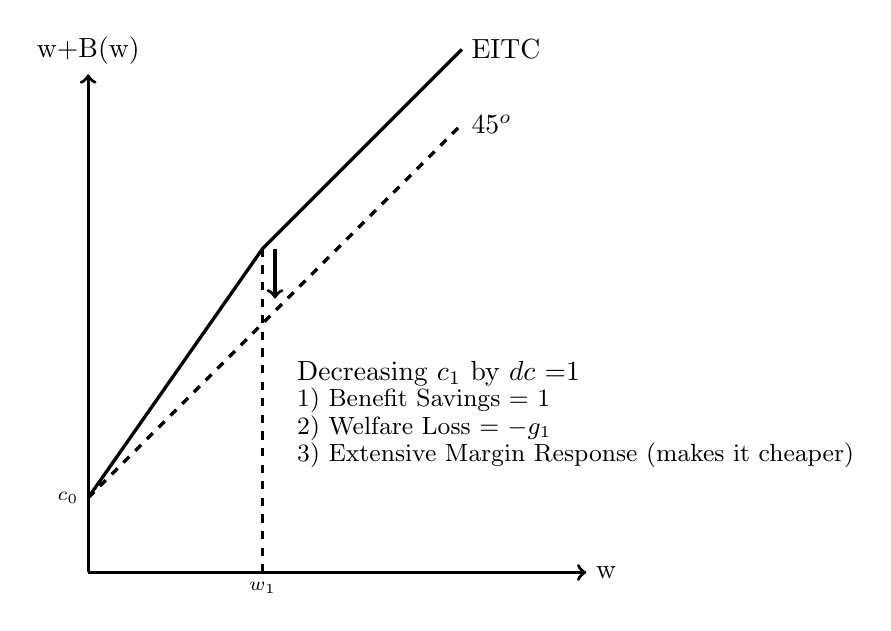
\begin{tikzpicture}[x=.9,y=.9]
\node[align=center, right] at (200,0) {w};
\draw[->, very thick] (0,0) -- (200,0) ; %edit here for the x axis
\node[align=center, above] at (0,200) {w+B(w)};
\draw[->, very thick] (0,0) -- (0,200) ; %edit here for the y axis

\draw[black, -, very thick] (0,30) -- (70,130) ; % 45 EITC
\draw[black, -, very thick] (70,130) -- (150, 210); % EITC
\node[black, align=center, right] at (150,210) {EITC};

\draw[black, -, dashed, thick] (70,0) -- (70,130) ;

\draw[->, very thick] (75,130) -- (75,110) ; %change

\draw[black, dashed, very thick] (0,30) -- (150,180) ; % 45 degree line
\node[black, align=center, right] at (150,180) {45$^o$};

\node[black, align=center, below] at (70,0) {\scriptsize{$w_1$}};

\node[black, align=right, left] at (0,30) {\scriptsize{$c_0$}};

\node[black, align=right, right] at (80,80) {Decreasing $c_1$ by $dc$ =1};
\node[black, align=right, right] at (80,69) {\small{1) Benefit Savings = 1}};
\node[black, align=right, right] at (80,58) {\small{2) Welfare Loss = $-g_1$}};
\node[black, align=right, right] at (80,47) {\small{3) Extensive Margin Response (makes it cheaper)}};
\end{tikzpicture}
\label{extensive_intuition}
\end{center}
\end{figure}
\end{frame}

\begin{frame}
\frametitle{Cost Minimizing}
\begin{figure}[H]
\begin{center}
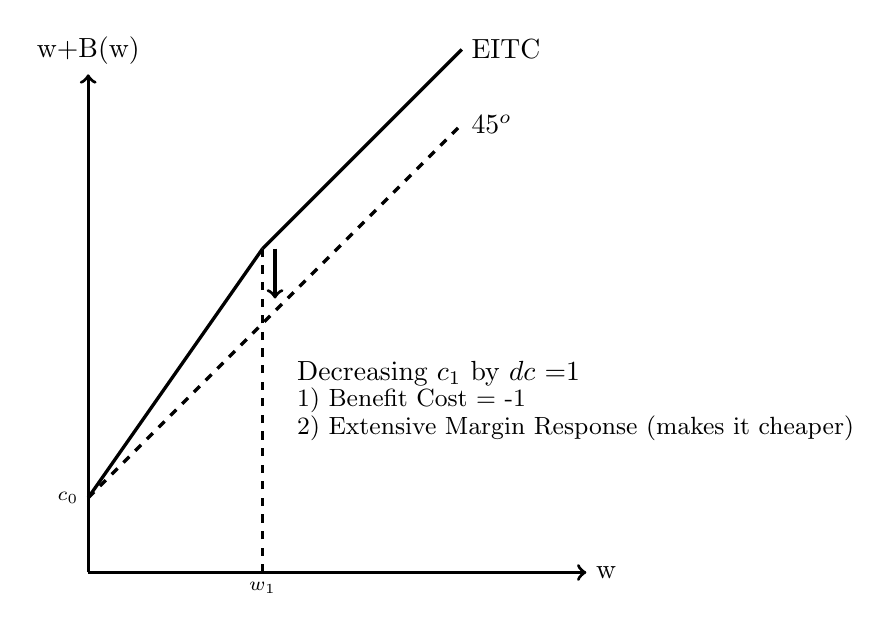
\begin{tikzpicture}[x=.9,y=.9]
\node[align=center, right] at (200,0) {w};
\draw[->, very thick] (0,0) -- (200,0) ; %edit here for the x axis
\node[align=center, above] at (0,200) {w+B(w)};
\draw[->, very thick] (0,0) -- (0,200) ; %edit here for the y axis

\draw[black, -, very thick] (0,30) -- (70,130) ; % 45 EITC
\draw[black, -, very thick] (70,130) -- (150, 210); % EITC
\node[black, align=center, right] at (150,210) {EITC};

\draw[black, -, dashed, thick] (70,0) -- (70,130) ;

\draw[->, very thick] (75,130) -- (75,110) ; %change

\draw[black, dashed, very thick] (0,30) -- (150,180) ; % 45 degree line
\node[black, align=center, right] at (150,180) {45$^o$};

\node[black, align=center, below] at (70,0) {\scriptsize{$w_1$}};

\node[black, align=right, left] at (0,30) {\scriptsize{$c_0$}};

\node[black, align=right, right] at (80,80) {Decreasing $c_1$ by $dc$ =1};
\node[black, align=right, right] at (80,69) {\small{1) Benefit Cost = -1}};
\node[black, align=right, right] at (80,58) {\small{2) Extensive Margin Response (makes it cheaper)}};
\end{tikzpicture}
\label{extensive_intuition}
\end{center}
\end{figure}
\hyperlink{prop_imp}{\beamergotobutton{Back to Proposition}}
\end{frame}

\begin{frame}[label=proof_relation]
\begin{proof}
Consider $dB_i=...=dB_I=dB$. 
The change in the cost of the program due to intensive margin responses in the discrete model is:
\begin{align*}
(B_{i-1}-B_i)dh_i-f_1de_i=[(1-\mu_{\bar{m}})dk_i+\mu_{\bar{m}} dh_i](B_{i-1}-B_i)=\\
[(1-\mu_{\bar{m}})\mathcal{E}_i^Rk_i+\mu_{\bar{m}}\mathcal{E}_ih_i]\frac{B_i-B_{i-1}}{w_i-w_{i-1}}\frac{dB}{c_i-c_{i-1}}(w_i-w_{i-1})
\end{align*}
In the continuous model, let $b_i=\frac{B_i-B_{i-1}}{w_i-w_{i-1}}$ and $f_i=\frac{p_{i-1}f_1}{w_i-w_{i-1}}$ be the marginal benefit and expected fines faced by individual with $\bar{y}=w_i$. The same perturbation $db_i=dB/(w_i-w_{i-1})$ will reduce the reported income of individuals reporting $w_i$ by $d\bar{y}=dy-d\tilde{y}$. So the tolal effect on cost is:
\begin{align*}
\{(1-\mu_{\bar{m}})[wi+\tilde{y}(w_i,m)]e_i+\mu_{\bar{m}}\bar{e}_i\}\frac{db_i}{1+b_i}h_ib_i
\end{align*}
Equating the terms multiplying $(1-\mu_{\bar{m}})$ and $\mu_{\bar{m}}$, we get the relations. 
\end{proof}
\hyperlink{discretized}{\beamergotobutton{Back to Discretized Schedule}}
\end{frame}

\setcounter{framenumber}{\value{finalframe}}

\end{document}
